\chapter{D\'eploiement}


\begin{figure}[ht]
	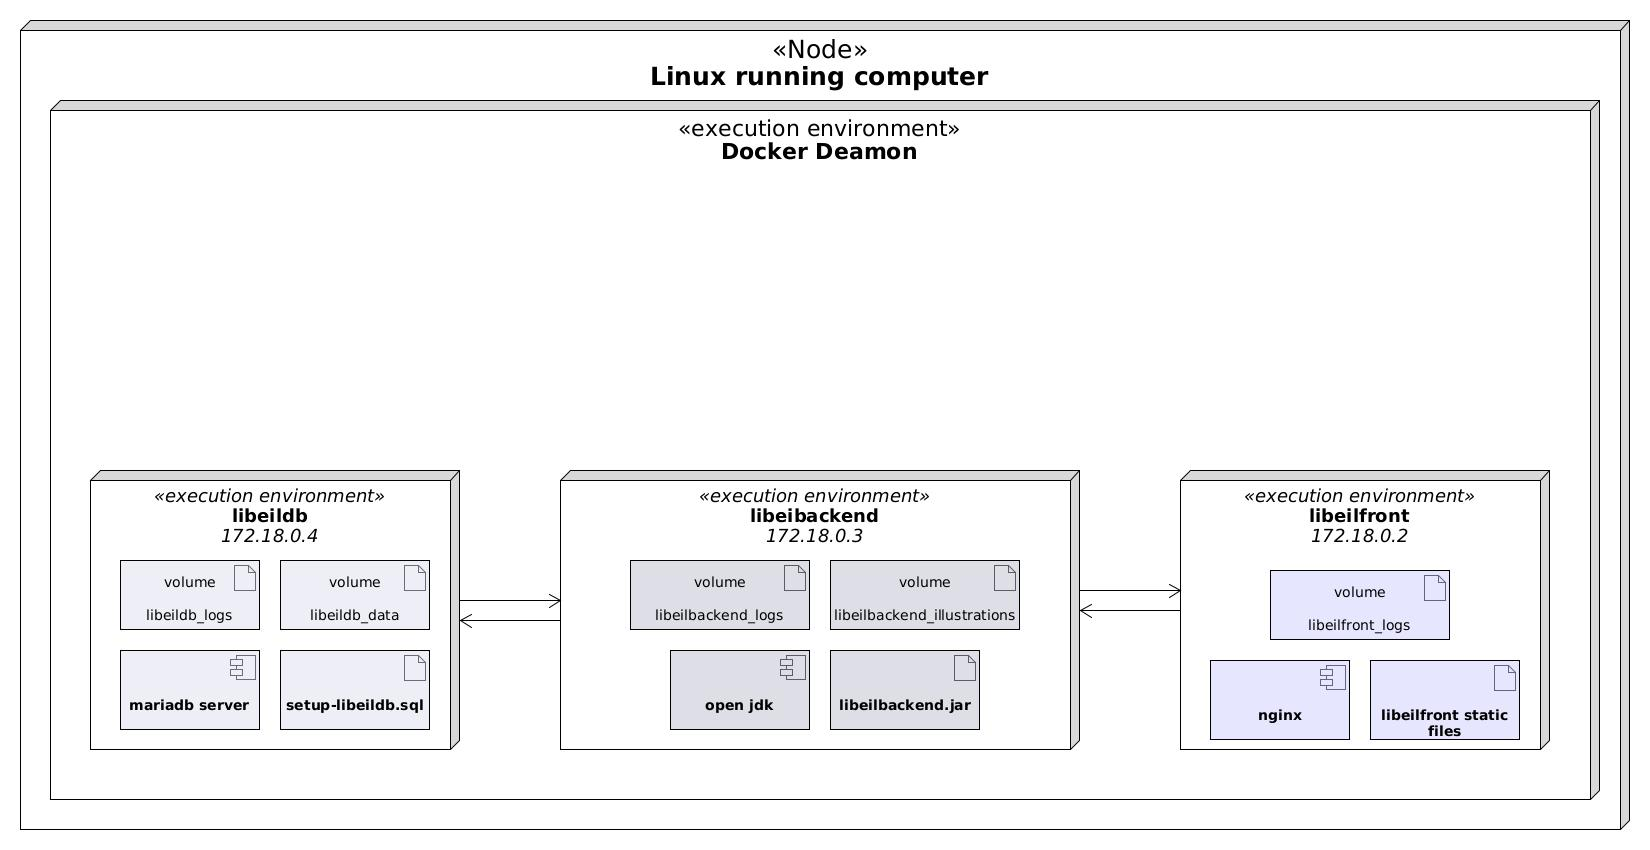
\includegraphics[width=0.75\textwidth]{Pictures/DiagrammeDeDeploiement.jpg}
	\centering
	\caption{Environnement de production.}
	\label{FigEnvironnementDeProduction}
\end{figure}

Le d\'eploiement est le processus qui, une fois la construction du site achet\'ee, permettra de la mettre en production. Dans notre cas, le d\'eploiement va consister \`a d\'efinir correctement l'environnement de production et \`a lancer les serveurs dans l'environnement d\'efini.


\section{Environnement de production}
\paragraph{} L'environnement de production d\'esigne ici l'ensemble form\'e d'un syst\`eme informatique qui fournit les ressources informatiques (Processeur, M\'emoire, Capacit\'e de stockage, ...) n\'ecessaires \`a l'ex\'ecution du site et d'une pile logicielle qui fournira les services dont le syst\`eme \`a besoin pour fonctionner (Syst\`eme d'exploitation, confidentialit\'e des donn\'ees, ...).

\subsection{Syst\`eme informatique}
Le syst\`eme informatique, suivant les besoins du site peut \^etre form\'e d'un ou de plusieurs ordinateurs et d'un ensemble de p\'eriph\'eriques.\\
Pour notre part, le syst\`eme informatique est un ordinateur physique ou virtuelle disposant d'assez de m\'emoire, d'espace de stockage, de d\'ebit r\'eseau, de CPU,... pour le fonctionnement de tout le site.


\subsection{Pile logicielle}
\subsubsection{Ubuntu}
Le premier logiciel est un syst\`eme d'exploitation. Nous utilisons Linux parce qu'en plus d'\^etre performant il est libre et open source par cons\'equent gratuit et fiable.

\paragraph{}De Linux, nous utilisons une distribution Ubuntu. Nous avons la derni\`ere version stable disponible.

\subsubsection{Docker Engine}
Docker est une technologie qui r\'evolutionne le d\'eveloppement et d\'eploiement de logiciels. Pour le d\'eploiement, Docker offre la possibilit\'e de lancer plusieurs applications sur un m\^eme ordinateur mais dans des environnements isol\'es les uns des autres.\\

L'application \textbf{Docker Engine} fournit une interface, et les service ad\'equates pour exploiter cette technologie.

\paragraph{} Nous utiliserons Docker pour pouvoir lancer les trois serveurs constituant le site sur un seul ordinateur.

\subsubsection{Nginx}
Pour assurer la disponibilit\'e de notre frontend sur le Web, nous devons utiliser un serveur Web. Les serveurs les plus connus et utilis\'es \`a cet effet sont \textbf{Apache} et \textbf{Nginx}.\\
Nous utilisons Nginx parce qu'il est plus efficace pour servir une front-end statique comme le notre et pour g\'erer une grande quantit\'e de trafique.







%\section{Protocole HTTPS}
%La s\'ecurit\'e du site est l'une des principales crit\`eres de qualit\'e de celui-ci. Elle consiste \`a garantir la disponibilit\'e, la confidentialit\'e et l'int\'egrit\'e des donn\'ees.\\ 
%HTTPS est une version s\'ecuris\'ee du protocole HTTP qui utilise SSL/TLS pour cripter les requ\^etes et r\'eponses HTTP classiques. Activer HTTPS sur le site le diminue les risques que les donne\'ees soient alt\'er\'ees au cours de leur transmission en contribuant ainsi \`a leur int\'egrit\'e. Cela emp\`eche qu'un hacker capte les paquets et d\'ecouvre acc\`ede au cr\'edential d'un administrateur et aux droit qui va avec. Donc il contribue \`a la confidentialit\'e des donn\'ees.			

%\paragraph{} Pour l'activer sur notre site, nous achetons un certificat SSL d'un vendeur et configurons Nginx pour utiliser le protocol s\'ecuris\'e de pr\'ef\'erence.


\section{Mise en production}
Une fois l'environnement de production op\'erationnel. Le site peut \^etre mis en production.

\subsection{Cr\'eation des images docker}
La premi\`ere \'etape consiste \`a cr\'eer une image docker pour chacun des trois serveurs.

\subsubsection{libeilfront}
L'image de l'interface utilisateur est bas\'ee sur la derni\`ere version alpine LTS (Long Time Support) du serveur web Nginx, \textbf{nginx:1.25.5-alpine}. On y cr\'ee un utilisateur non-root et un nouveau groupe pour notre utilisateur en sorte que Nginx ne soit pas lanc\'e en tant qu'administrateur, ce qui repr\'esenterait un risque pour la s\'ecurit\'e du site. Enfin on y copie les fichiers statiques provenant de l'application front-end d\'evelopp\'ee sur angular.

\subsubsection{libeilbackend}
L'image du serveur d'application est bas\'ee sur \textbf{openjdk:19-jdk-alpine}. On y cr\'ee un utilisateur non-root et un nouveau groupe pour notre utilisateur. Ensuite on y copie le package JAR (\textit{libeilbackend.jar}) de l'application d\'evelopp\'ee avec Spring Boot.

\subsubsection{libeildb}
L'image de la base de donn\'ees est bas\'ee sur \textbf{mariadb:10.11.6}. On y copie le script libeildb-setup.sql pour assurer la cr\'eation de la base une fois l'image lanc\'ee.

\subsection{Docker compose}
Docker compose permet de lancer les trois images comme une seule application. Pour cela nous cr\'eons un service pour chaque serveur bas\'e sur l'image ad\'equat. Nous cr\'eons aussi un r\'eseau priv\'e auquel nous ajoutons tous les services tout en leur donnant une adresse sur le r\'eseau priv\'e. En dernier lieu nous d\'efinissons des volumes pour garantir la persistance \`a la fois des donn\'ees de la base et des fichiers d'une part, et pour monter des fichiers de configuration aux conteneurs des diff\'erents services.\\

\subsection{+}
De l\`a, il suffit de lancer le fichier docker-compose.yml et l'application est en production



